% !TeX spellcheck = cs_CZ
%{\tikzset{external/prefix={tikz/FYZI/}}
% \tikzset{external/figure name/.add={ch05_}{}}
%---------------------------------------------------------------------------------------------------
% file fey1ch07.tex
%---------------------------------------------------------------------------------------------------
%================ Kapitola: Teorie gravitace =======================================================
\setchaptertoc
\chapter{Teorie gravitace}\label{fyz:chap_fey_gravity}

  \section{Úvod}
    Gravitační interakce je jediná interakce, která působí na všechny objekty ve vesmíru. Není
    výběrová. Jde o interakci, která výraznou měrou určuje strukturu vesmíru. První velké úspěchy
    při poznání gravitace slavil Isaac Newton. Objevil univerzální gravitační zákon, podle kterého
    padají předměty na Zemi, pohybuje se Měsíc kolem Země, planety kolem Slunce a kterým se řídí i
    ohromné hvězdné ostrovy, kterým říkáme galaxie. Ve Sluneční soustavě, ale i jinde, existují
    energeticky výhodné dráhy, klikaté koridory, které propojují Lagrangeovy body, v nichž se
    všechny síly vyrovnávají. Pokud se vesmírná sonda pohybuje po takové gravitační superdálnici,
    spotřebuje minimální množství paliva.

    \begin{figure}[ht!] %\ref{fyz:fig0886}
      \centering
      \luafigure[1]{fyz_fig0886.jpg}
      \caption{Simulace gravitační superdálnice. Kredit: NASA/JPL. }
      \label{fyz:fig0886}
    \end{figure}

    Přesto Newtonův gravitační zákon selhává při silných polích a vysokých rychlostech částic. Není
    v něm zabudována rychlost šíření interakce a není relativistický. Dnešní obecná relativita
    pracuje s časoprostorem, který tělesa svou přítomností zakřivují a v němž se pohybují po
    nejrovnějších možných drahách. Nové pojetí gravitace předpovídá mnohé nové jevy: dráhy těles
    kolem hmotného centra již nejsou elipsy, světlo se v křivém časoprostoru ohýbá, existují
    gravitační čočky, existují zkolabované hvězdy - černé díry, vesmír jako celek expanduje a
    objekty s nenulovým kvadrupólovým momentem vyzařují gravitační vlny. V současnosti se připravují
    fascinující experiementy, které by mohly polapit i gravitační vlny ze samotného vzniku vesmíru.

  \section{Pohyb planet}
    Vraťme se do doby, kdy \emph{Galileo Galilei} (1564-1642) provedl své první gravitační
    experimenty. Gelileo byl toskánský astronom a fyzik těsně spjatý s vědeckou revolucí. Sledoval
    volný pád, šikmý vrh, pohyb po nakloněné rovině a závislost periody kyvadla na délce závěsu.
    Objevil základní zákony těchto pohybů, včetně zákona o skládání rychlostí. Poprvé v novodobých
    dějinách použil experiment k ověření myšlenkových konstrukcí. Kromě těchto aktivit byl také
    konstruktérem prvního astronomického dalekohledu, objevil krátery na Měsíci, Jupiterovy měsíce
    Io, Europu, Ganymedes a Callisto a sledoval Mléčnou dráhu.

    Budeme hovořit o jednom z nejdalekosáhlejších zobecnění, které lidská mysl uskutečnila. Měli
    bychom však postát s úctou před přírodou, která tak dokonale splňuje skvělý a jednoduchý
    princip, jakým je gravitační zákon. Co to je, ten gravitační zákon? Vyjadřuje skutečnost, že
    každý předmět ve vesmíru přitahuje kterýkoli jiný předmět silou, která je pro libovolná dvě
    tělesa úměrná hmotnosti každého z nich a mění se nepřímo úměrně čtverci vzdálenosti mezi nimi.
    Tento výrok lze matematicky vyjádřit vztahem
    \begin{equation}\label{fyz:eq096}
      \boxed{F = \kappa\frac{m_1m_2}{r^2}}
    \end{equation}
    Uvedeme-li navíc skutečnost, že předmět reaguje na sílu zrychlením ve směru působení síly a 
    velikost zrychlení je nepřímo úměrná hmotnosti předmětu, poskytli jsme všechny potřebné 
    informace a dostatečně nadaný matematik je schopen odvodit všechny důsledky těchto dvou 
    principů.
    
    Zatím však nejsme dostatečně pokročilí, a proto budeme o důsledcích hovořit podrobněji a 
    nezůstaneme jen u samotných principů. Stručně připomeneme historii objevu gravitačního zákona a 
    pohovoříme o některých jeho důsledcích, jeho vlivu na historii, o záhadách, které se za tímto 
    zákonem skrývají a o tom, jak ho upřesnil Einstein. Budeme hovořit i o jeho vztahu k jiným 
    fyzikálním zákonům. Všechno však není možné stihnout v jedné kapitole, proto uvedeným problémům 
    věnujeme i následující kapitoly.

    \begin{figure}[ht!]  %\ref{fyz:fig0299}
      \centering
      \luafigure[1]{fyz_fig0299.pdf}
      \caption{Dráha planety Mars, po níž se pohybovala na pozadí souhvězdí Kozoroha během roku 
               1971. Na obrázku je znázorněna jeho poloha ve čtyřech různých dnech.Planety Marsi 
               Země se obě pohybují po oběžných drahách kolem Slunce; zde vidíme polohu Marsu 
               vzhledem k Zemi.Díky tomu pozorujeme na dráze Marsu zdánlivé smyčky. 
               (\cite[s.~366]{Halliday2001})}
      \label{fyz:fig0299}
    \end{figure}
    
    Historie začíná u našich dávných předků, kteří pozorovali pohyb planet mezi hvězdami a nakonec 
    usoudili, že planety se pohybují kolem Slunce, což později znovu objevil Koperník. Trochu více 
    úsilí si vyžadovalo poznání toho, jak se planety kolem Slunce pohybují, jak jejich pohyb přesně 
    probíhá. Například smyčkovitý pohyb Marsu, znázorněný na obr. \ref{fyz:fig0299}, byl obzvláště 
    matoucí.
   
    Na začátku patnáctého století se hodně diskutovalo o tom, jestli se planety opravdu pohybují 
    kolem Slunce nebo ne. Tycho Brahe (1546-1601) přišel se zcela novou myšlenkou. Spočívala v tom, 
    že tyto diskuse mohou vyřešit jen dostatečně přesná měření poloh planet na obloze. Ukáží-li 
    měření přesně, jak se planety pohybují, pak snad bude možné rozhodnout se pro jedno nebo druhé 
    stanovisko. Byla to úžasná myšlenka - že něco je lépe poznávat cestou pečlivých experimentů než 
    pokračováním v hlubokých filozofických úvahách. Při uskutečňování této myšlenky sledoval Tycho 
    Brahe ve své observatoři na ostrově Hven u Kodaně po dlouhá léta pohyby planet. Vyhotovil 
    rozsáhlé tabulky, které po jeho smrti studoval matematik \emph{Johannes Kepler} (1571-1630). 
    Kepler na základě těchto údajů objevil některé krásné, pozoruhodné a přitom jednoduché zákony 
    planetárního pohybu. Později ukázal Newton (1642-1727), že z jeho gravitačního zákona lze 
    Keplerovy empirické zákony odvodit i teoreticky.

    \begin{figure}[ht!]  %\ref{fyz:fig0887}
      \centering
      \luafigure[1]{fyz_fig0887.jpg}
      \caption{Korifejové klasické gravitační teorie: Galileo Galilei (1564-1642), Tycho Brahe
               (1564-1642), Johannes Kepler (1571-1630) a Isaac Newton (1643-1727). Kredit:
               Aldebaran}
      \label{fyz:fig0887}
    \end{figure}

    
  \section{Keplerovy zákony}
    Kepler především zjistil, že každá planeta obíhá kolem Slunce po křivce nazývané 
    \textbf{elipsa}, přičemž Slunce se nachází v ohnisku elipsy. To je obsah \textbf{prvního 
    Keplerova} zákona. Elipsa není prostý ovál, ale představuje velmi svéráznou, přesné definovanou 
    křivku, kterou je možné získat tak, že tužkou napínáme nit upevněnou na dvou špendlíčkách 
    umístěných v ohniscích. Kdybychom se chtěli vyjádřit matematicky, museli bychom říci, že jde o 
    \emph{geometrické místo bodů, které mají stálý součet vzdáleností od dvou pevných bodů 
    (ohnisek)}. Nebo jestli se nám to líbí, je to kružnice, na kterou se díváme ze strany (obr. 
    \ref{fyz:fig0062}).
    
    \begin{figure}[ht!]  %\ref{fyz:fig0062}
      \centering
      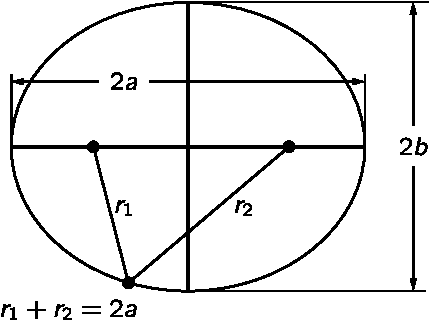
\includegraphics[width=0.5\linewidth]{fyz_fig0062.pdf}
      \caption{Elipsa (\cite[s.~93]{Feynman01})}
      \label{fyz:fig0062}
    \end{figure}
    \textbf{Druhým Keplerovým} poznatkem bylo zjištění, že planety neobíhají kolem Slunce stálou 
    rychlostí. Když jsou ke Slunci blíže, pohybují se rychleji, a když jsou od něho vzdálenější, 
    pohybují se pomaleji. Přesně můžeme tento pohyb popsat následujícím způsobem. Předpokládejme, 
    že pozorujeme planetu ve dvou po sobě jdoucích časových okamžicích, například časově vzdálených 
    o týden, a zakreslujeme průvodiče\footnote{Průvodič je úsečka spojující Slunce s kterýmkoliv 
    bodem na planetární dráze.} planety pro každou pozorovanou polohu. Přesně můžeme tento pohyb 
    popsat následujícím způsobem. Dráhový oblouk, který planeta prošla po týdnu a dva průvodiče 
    vymezují určitou plochu. Tato plocha představuje vyšrafovanou oblast na obr. \ref{fyz:fig0063}. 
    Uskuteční-li se i druhé takové týdenní pozorování, a to tehdy, kdy je planeta dále od Slunce (a 
    má tedy menší rychlost), podobným způsobem vymezená plocha je přesné stejná, jako v 
    předcházejícím případě. \emph{Druhý Keplerův zákon tedy říká, že každá planeta obíhá kolem 
    Slunce takovou rychlostí, že plochy opsané průvodičem za stejnou dobu jsou stejné!}
    
    \begin{figure}[ht!]  %\ref{fyz:fig0063}
      \centering
      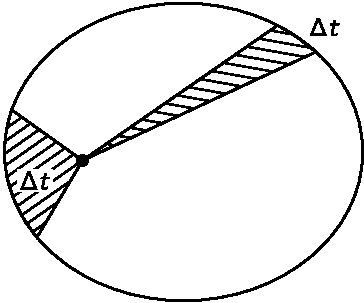
\includegraphics[width=0.5\linewidth]{fyz_fig0063.pdf}
      \caption{Keplerův zákon ploch (\cite[s.~94]{Feynman01})}
      \label{fyz:fig0063}
    \end{figure}
    \textbf{Třetí zákon} Kepler objevil mnohem později a patří do jiné kategorie než první dva, 
    neboť nehovoří jen o jedné planetě, ale dává do souvislosti jednotlivé planety. Tento zákon 
    porovnává periody (oběžné doby) a rozměry drah jednotlivých planet a říká, že periody jsou 
    úměrné \sfrac{3}{2} mocnině rozměrů drah. Periodou rozumíme dobu, který planeta potřebuje k oběhu 
    celé dráhy a rozměr se určuje délkou největšího průměru eliptické dráhy, známého jako 
    \emph{hlavní osa}. Kdyby se planety pohybovaly po kružnicích (a tato představa je dost blízko 
    skutečnosti), čas potřebný k opsání kružnice by byl úměrný \sfrac{3}{2} mocnině průměru (nebo 
    poloměru) kružnice. \textbf{Keplerovy zákony} tedy zní:
    
    \begin{enumerate}[noitemsep]
      \item Každá planeta se pohybuje kolem Slunce po elipse, přičemž Slunce je v jednom z ohnisek.
      \item Průvodič spojující Slunce s planetou opisuje stejné plochy za stejné časové intervaly.
      \item Druhé mocniny period libovolných dvou planet jsou úměrné třetím mocninám velkých poloos 
            jejich drah \(T\approx a^\frac{3}{2}\).
    \end{enumerate}
    
  \section{Rozvoj Dynamiky}
    V době, kdy Kepler objevoval tyto zákony, Galileo se zajímal o zákony pohybu. Bylo třeba 
    objasnit, co nutí planety se pohybovat. (V té době jedna z „teorií“ planetárního pohybu 
    předpokládala, že příčinou pohybu planet jsou neviditelní andělé, kteří máváním svých křídel 
    tlačí planety dopředu v oběhu. Uvidíte, že dnes je již tato teorie pozměněná! Ukazuje se, že k 
    udržení planet musí neviditelní andělé působit na planety v jiném směru a nemají křídla. V 
    ostatním jsou však obě teorie podobné!) Galileo objevil pozoruhodnou vlastnost pohybu, jež byla 
    podstatnou pro pochopení těchto zákonů. Jde o \textbf{princip setrvačnosti} - jestliže se něco 
    pohybuje tak, že není s ničím ve styku a nic ho neruší, pak se bude pohybovat nepřetržitě podél 
    přímky a jeho rychlost bude \emph{konstantní}. (Proč pohyb neustane, to nevíme. Víme však, že 
    je to tak.)
    
    Newton upravil tuto myšlenku, když říkal, že jediným způsobem jak změnit pohyb tělesa je použít 
    \textbf{sílu}. Když se pohyb tělesa zrychluje, musela síla působit ve směru pohybu. Na druhé 
    straně, jestliže se změnil směr pohybu tělesa, síla působila ze strany. Newton tedy doplnil 
    tuto myšlenku o poznatek, že síla je potřebná ke změně velikosti rychlosti nebo směru pohybu 
    tělesa. Například, upevníme-li kámen na provaz a roztáčíme ho po kruhové dráze, potřebujeme 
    sílu, abychom ho na této dráze udrželi. Musíme tahat za provaz. Zákon ve skutečnosti říká, že 
    zrychlení vyvolávané silou je nepřímo úměrné hmotnosti tělesa, nebo, že síla je úměrná součinu 
    hmotnosti a zrychlení. Čím je těleso hmotnější, tím větší síla je potřebná k dosažení daného 
    zrychlení tělesa. (Hmotnost je možné měřit tak, že na konec stejného provazu upevňujeme různé 
    kameny a nutíme je pohybovat se po stejné kruhové dráze stejnou rychlostí. Tak zjistíme, že k 
    tomu je třeba větší nebo menší síly. Předměty vyžadující větší sílu, mají větší hmotnost.)
    
    Z těchto úvah vyplývá velkolepá myšlenka, že k udržení planet na jejich drahách nejsou potřebné 
    \emph{tangenciální síly} (andělé nemusí letět ve směru tečny), protože planeta i tak poletí v 
    daném směru. Kdyby planetu nic nerušilo, odletěla by \emph{přímočaře}. Skutečný pohyb se však 
    odchyluje od přímky, po níž by se těleso pohybovalo v nepřítomnosti sil, a tato odchylka je 
    \emph{kolmá} ke směru pohybu - tedy ne ve směru jeho pohybu. Jinými slovy: v důsledku principu 
    setrvačnosti není síla potřebná k udržení pohybu planet \emph{kolem} Slunce silou směřující 
    kolem Slunce, ale silou směřující ke Slunci. (Existuje-li tu síla směřující ke Slunci, může být 
    Slunce, samozřejmě, oním andělem!)
    
  \section{Newtonův gravitační zákon}
    Newton dokonaleji pochopil teorii pohybu a tak dospěl k přesvědčení, že \emph{právě Slunce} by 
    mohlo být místem nebo původcem sil, jež ovládají pohyb planet. Podařilo se mu dokázat (možná, 
    že to brzy dokážeme i my), že opisování stejných ploch za stejnou dobu znamená, že všechna 
    odchýlení od přímočarého pohybu jsou přesně \emph{radiální} - že zákon je přímým následkem 
    toho, že všechny síly \emph{směřují ke Slunci}
    
    Dále je možné analýzou třetího Keplerova zákona dokázat, že čím dále je planeta od Slunce, tím 
    jsou síly menší. Porovnáme-li dvě planety, různě vzdálené od Slunce, zjistíme, že síly jsou 
    nepřímo úměrné druhé mocnině odpovídajících vzdáleností. Kombinováním těchto dvou zákonů 
    usoudil Newton, že existuje síla, která je nepřímo úměrná druhé mocnině vzdálenosti a směřuje 
    po přímce, jež prochází dvěma na sebe působícími objekty.
    
    Newton, jenž měl značný smysl pro zobecnění, samozřejmě předpokládal, že tento vztah neplatí 
    jen pro Slunce přitahující planety. Tehdy se již například vědělo, že planeta Jupiter má 
    měsíce, které ji obíhají tak, jako zemský Měsíc obíhá Zemi a Newton si byl jistý, že každá 
    planeta přidržuje silou svůj měsíc ve své blízkosti. Newton již znal sílu, jež nás přidržuje na 
    Zemi, a tak předpokládal, že jde o \emph{univerzální} sílu - \emph{že vše je přitahováno vším}.
    
    Dále ho zajímalo, zda Země přitahuje stejnou silou lidi i Měsíc, tj. silou, jež je nepřímo 
    úměrná druhé mocnině vzdálenosti. Padá-li předmět na zemském povrchu \qty{5}{\m} za první 
    sekundu po vypuštění, o jakou vzdálenost spadne Měsíc za stejnou dobu? Je možné namítnout, že 
    Měsíc vůbec nepadá. Kdyby však na Měsíc nepůsobila síla, odletěl by po přímce, zatímco se 
    pohybuje po kružnici, takže skutečně padá z místa, na kterém by byl, kdyby na něj nepůsobily 
    síly. Protože známe poloměr jeho oběžné dráhy (asi \qty{380000}{\km}) a dobu oběhu Měsíce kolem 
    Země (přibližně \num{29} dní), můžeme vypočítat, jakou vzdálenost urazí Měsíc za \num{1} 
    sekundu a pak, o kolik za tuto dobu klesne\footnote{Tj. jak se kružnice oběžné dráhy Měsíce 
    odkloní od své tečny na úseku, který Měsíc urazí za 1 sekundu.}. Tato vzdálenost je přibližně 
    rovna \qty{1.4}{\mm} za sekundu. To zcela souhlasí se \emph{zákonem reciprokých čtverců}, neboť 
    zemský poloměr je roven \qty{6380}{\km} a padá-li v této vzdálenosti těleso o \qty{5}{\m} za 
    první sekundu, pak ve vzdálenosti \qty{380000}{\km}, tedy \num{60}-krát větší, by mělo spadnout 
    jen \sfrac{1/3600} z \qty{5}{\m}, což je zhruba \qty{1.4}{\mm}. Podobnými výpočty Newton prověřoval 
    svou gravitační teorii. Výpočty provedl velmi pečlivě a zjistil tak velké odchylky, že 
    považoval teorii za protiřečící faktům a své výsledky nepublikoval. Po šesti letech byla 
    provedena nová měření zemských rozměrů, která ukázala, že astronomové používali nesprávnou 
    vzdálenost k Měsíci. Jakmile se o tom Newton doslechl, provedl své výpočty s opravenými údaji a 
    dospěl k překrásné shodě. Tj. jak se kružnice oběžné dráhy Měsíce odkloní od své tečny na 
    úseku, který Měsíc urazí za \num{1} sekundu.
    
    Myšlenka, že Měsíc „padá“, vyvolává rozpaky, neboť jak vidíme, Měsíc se k nám nepřibližuje. 
    Tato myšlenka je tak zajímavá, že si zasluhuje další vysvětlení: Měsíc padá v tom smyslu, že se 
    \emph{odklání od přímky, po níž by se pohyboval v nepřítomnosti sil}. Všimněme si příkladu ze 
    zemského povrchu. Předmět vypuštěný v blízkosti zemského povrchu padá \qty{5}{\m} za první 
    sekundu. I předmět vystřelený horizontálně spadne \qty{5}{\m}; ačkoli se pohybuje 
    \emph{horizontálně}, přece spadne za stejný čas o \qty{5}{\m}. Na obr. \ref{fyz:fig0058} je 
    znázorněno zařízení na ověření této skutečnosti. Na horizontálním žlábku je míček, který se 
    bude pohybovat dopředu. Ve stejné výšce je míček, který bude padat vertikálně, přičemž 
    elektrický spínač je nastaven tak, že v okamžiku, kdy první míček opouští žlábek, uvolňuje se 
    druhý míček. Důkazem toho, že za stejnou dobu spadnou stejně hluboko, je jejich srážka ve 
    vzduchu.
    
    \begin{figure}[ht!]  %\ref{fyz:fig0058}
      \centering
      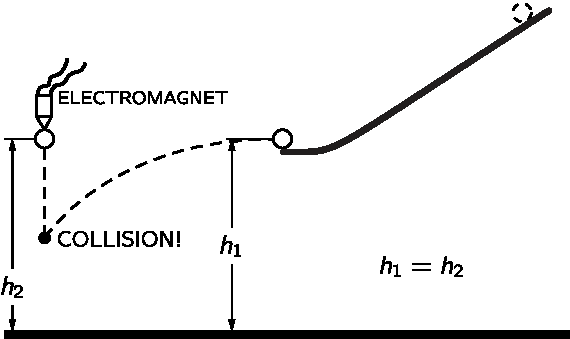
\includegraphics[width=0.6\linewidth]{fyz_fig0058.pdf}
      \caption{Zařízení na demonstraci nezávislosti horizontálního a vertikálního pohybu 
               (\cite[s.~96]{Feynman01})}
      \label{fyz:fig0058}
    \end{figure}
    Kulka vystřelená horizontálně, může za \num{1} sekundu proletět velkou vzdálenost - snad půl 
    kilometru - ale za ten čas spadne vždy o \qty{5}{\m}, byla-li vystřelená skutečně horizontálně. 
    Co se bude dít, budeme-li kulku vystřelovat rychleji a rychleji? Nesmíme zapomenout, že zemský 
    povrch je zakřivený. Vystřelíme-li kulku dostatečně rychle, může se stát, že ačkoli spadne o 
    \qty{5}{\m}, zůstane ve stejné výšce nad zemí, jako byla předtím. Jak je to možné? Ačkoli kulka 
    padá, Země se zakřivuje a tak se stává, že kulka padá \uv{kolem} Země. Je však třeba odpovědět 
    na otázku, jak daleko se musí dostat kulka za jednu sekundu, aby země byla \qty{5}{\m} pod 
    horizontem. Na obr. \ref{fyz:fig0059} je znázorněna Země s jejím \qty{6380}{\km} dlouhým 
    poloměrem a tečna - přímka, po níž by se kulka pohybovala v nepřítomnosti sil. Použijeme-li 
    jednu z nádherných geometrických pouček, která říká, že naše tečna je geometrický průměr dvou 
    částí průměru vyťatých stejně dlouhou tětivou, zjistíme, že horizontální vzdálenost, kterou 
    kulka urazí, je geometrický průměr z \qty{5}{\m} pádu a \qty{12760}{\km} zemského průměru. Druhá 
    odmocnina z (\(\num{0.005}\times\num{12760}\)) vychází přibližně \qty{7.9}{\km}. Pohybuje-li se 
    tedy kulka rychlostí \qty{7.9}{\km} za sekundu, bude padat k Zemi každou sekundu o \qty{5}{\m}, 
    ale nikdy se k Zemi nepřiblíží, neboť Země je zakřivená. Tak to bylo i s Gagarinem, který 
    obíhal Zemi rychlostí přibližně \qty{8}{\km/\second} po \qty{40000}{\km} dlouhé oběžné dráze. (Ve 
    skutečnosti trochu více, neboť letěl výše.)

    \begin{figure}[ht!]  %\ref{fyz:fig0089}
      \centering
      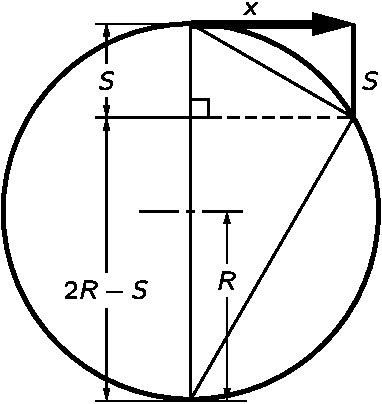
\includegraphics[width=0.4\linewidth]{fyz_fig0059.pdf}
      \caption{Dostředivé zrychlení při kruhové dráze. Z podobnosti trojúhelníku: \(\frac{x}{s} = 
               \frac{(2R - s)}{x} \approx \frac{2R}{x}\) kde \(R\) je poloměr Země             
               (\qty{6380}{\km}), \(x\) je vzdálenost „prošlá horizontálně a za jednu sekundu a
               \(s\) je vzdálenost \uv{padání} za jednu sekundu (přibližně \qty{5}{\m})
               \cite[s.~97]{Feynman01}}
       \label{fyz:fig0059}
    \end{figure}
    
    Každý objev nového zákona je užitečný jen tehdy, když je z něho možné získat více, než bylo do 
    něho vloženo. Newton použil druhý a třetí Keplerův zákon k odvození svého gravitačního zákona. 
    Co předpověděl? Nejdříve to byla jeho analýza pohybu Měsíce, neboť dávala do souvislosti padání 
    předmětů na Zemi s \uv{padáním} Měsíce. Druhou předpovědí byla odpověď na otázku, zda jsou 
    dráhy planet elipsy. Později uvidíme, jak je možno přesně vypočítat tento pohyb a dokázat, že 
    planety se skutečně pohybují po elipsách. Takže žádná jiná fakta k důkazu prvního Keplerova 
    zákona nepotřebujeme. Tak Newton uskutečnil svou první velkou předpověď.

    Gravitační zákon vysvětluje mnoho dříve nepochopených jevů, například do té doby záhadný jev 
    \textbf{slapových pohybů} - \emph{přílivu a odlivu} - způsobovaných měsíční přitažlivostí. Lidé 
    se i předtím domnívali, že Měsíc přitahuje vodu pod sebou a způsobuje příliv, ale nebyli tak 
    bystří jako Newton, a proto si mysleli, že by měl být jen jeden příliv za den. Předpokládalo 
    se, že Měsíc přitahuje vodu a vyvolává tak příliv a odliv a protože se Země otáčí, měl by v 
    každém místě nastat příliv a odliv za \num{24} hodin. Skutečnost je však taková, že příliv a 
    odliv nastávají každých \num{12} hodin. Podle jiných představ měl zase příliv nastat na opačné 
    straně Země, neboť Měsíc odtahuje Zemi od vody! Obě dvě tyto teorie jsou nesprávné. Proces 
    probíhá následujícím způsobem: měsíční přitažlivost Země i vody je ve středu Země, v průměru 
    vyvážená. Avšak voda, která je blíže k Měsíci, je přitahována více než je průměrná 
    přitažlivost, zatímco voda na vzdálenější straně je přitahována méně než je průměrná 
    přitažlivost. Navíc, voda může téct, zatímco pevná Země ne. To, co skutečně pozorujeme, je pak 
    kombinace těchto dvou úkazů.

    \begin{figure}[ht!]  %\ref{fyz:fig0060}
      \centering
      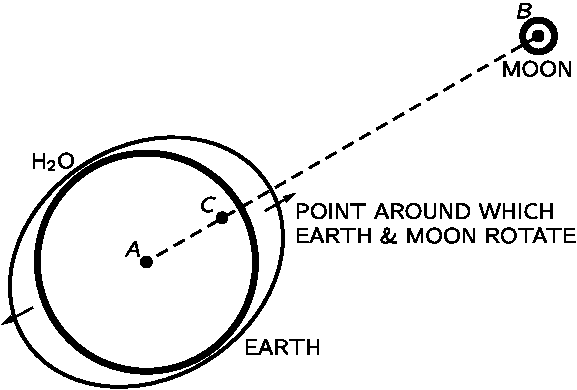
\includegraphics[width=0.7\linewidth]{fyz_fig0060.pdf}
      \caption{Slapové pohyby v soustavě Země - Měsíc (\cite[s.~97]{Feynman01})}
      \label{fyz:fig0060}
    \end{figure}
    Co chápeme pod slovem „vyvážený“? Co je vyvážené? Přitahuje-li Měsíc celou Zemi, proč ta 
    nespadne „nahoru“ na Měsíc? Ze stejné příčiny, ze které Měsíc nespadne na Zemi. Země obíhá 
    kolem bodu, jenž leží v jejím nitru, ale není v jejím středu. Měsíc neobíhá jen kolem Země, ale 
    Země i Měsíc obíhají kolem centrální polohy a obě tělesa padají na toto společné centrum, jak 
    je to znázorněno na obr. \ref{fyz:fig0060}. Tento pohyb kolem společného centra je tím, co 
    vyvažuje pád každého z těchto těles. Ani Země se tedy nepohybuje po přímce, ale po kružnici. 
    Voda na vzdálenější straně je „nevyvážená“, neboť vjejím místě je měsíční přitažlivost slabší 
    než ve středu Země, kde vyvažuje „odstředivou“ sílu. Výsledkem této nevyváženosti je, že voda 
    se zvedá směrem od středu Země. Na bližší straně je měsíční přitažlivost silnější a 
    nevyváženost má opačný směr v prostoru, ale opět směřuje pryč od středu Země. Výsledkem je 
    existence dvou přílivových vzdutí.
    
  \section{Všeobecná gravitace}
    Co ještě můžeme pochopit, známe-li gravitaci? Každý ví, že Země je kulatá. Proč je Země kulatá? 
    To je jednoduché; následkem gravitace. Země je kulatá proto, že všechno se navzájem přitahuje a 
    tak se to, z čeho Země vznikla, přitahovalo, dokud to bylo možné! Chceme-li být přesnější, Země 
    není přesná koule, neboť rotuje a tato rotace vede k odstředivému působení, jež zmenšuje 
    gravitační působení v blízkosti rovníku. Země by tedy měla být elipsoidem, jehož přesný tvar 
    dokonce umíme určit. Z gravitačního zákona tedy můžeme usoudit, že Slunce, Měsíc i Země by měly 
    mít (přibližně) kulový tvar.
    
    Co ještě můžeme určit z gravitačního zákona? Podíváme-li se na měsíce Jupitera, pochopíme vše o 
    způsobu jejich pohybu kolem této planety. Mimochodem, jednou byl problém právě s měsíci 
    Jupitera a nebude od věci něco si o tom říci. Tyto měsíce velmi podrobně studoval Roemer a 
    všiml si, že někdy předbíhají \uv{letový řáď} a někdy se zase opožďují. (Jejich \uv{letový řáď} 
    je možné sestavit po velmi dlouhém pozorování zjištěním průměrné doby obletu.) Měsíce 
    předbíhaly řád, když byl Jupiter obzvláště blízko k Zemi a opožďovaly se, když byl Jupiter 
    vzdálený od Země. Je to velmi těžké vysvětlit podle gravitačního zákona - dokonce by to mohlo 
    pohřbít tuto nádhernou teorii, kdyby neexistovalo jiné vysvětlení. Kdyby totiž zákon 
    nevyhovoval třeba jen v jednom případě, v němž by měl platit, byl by nesprávný. Tento rozpor se 
    však dal vysvětlit velmi jednoduše a krásně: K tomu, abychom pozorovali měsíce Jupitera, je 
    potřebný určitý čas, za který světlo urazí vzdálenost od Jupitera k Zemi. Je-li Jupiter 
    \emph{blíže} k Zemi, čas je \emph{kratší} a je-li Jupiter \emph{dále}, čas je \emph{delší}. 
    Proto se měsíce zdánlivě jednou předbíhají a jindy opožďují za letovým řádem, podle toho, zda 
    jsou blíže nebo dále od Země. Tento úkaz, který svědčí o tom, že světlo se nešíří okamžitě, 
    poskytl první odhad rychlosti šíření světla. Bylo to roku 1656.
    
    \begin{figure}[ht!]  %\ref{fyz:fig0089}
      \centering
      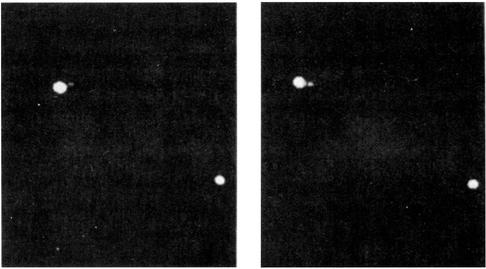
\includegraphics[width=0.8\linewidth]{fyz_fig0089.jpg}
      \caption{Systém dvojhvězdy (\cite[s.~99]{Feynman01})}
      \label{fyz:fig0089}
    \end{figure}
    

    Při\-ta\-hují-li se vzájemně všechny planety, pak síla, která ovládá například Jupiter na jeho 
    cestě kolem Slunce, nepochází jen od Slunce; pochází například i od Saturnu. Ačkoli tato síla 
    není velká, neboť Slunce má mnohem větší hmotnost než Saturn, přece to je jen určitá síla a 
    dráha Jupitera by neměla být - a ani není - dokonalou elipsou; je trochu vychýlená a 
    \uv{kolísá} kolem skutečně eliptické dráhy. Takový pohyb je trochu komplikovanější. Byly 
    uskutečněny pokusy o analýzu pohybu Jupitera, Saturnu a Uranu na základě gravitačního zákona. 
    Započítaly se vlivy jednotlivých planet, aby se zjistilo, jestli tento zákon vysvětluje drobné 
    odchylky a nepravidelností v jejich pohybu. A hle - v případě Jupitera a Saturnu bylo vše v 
    pořádku, ale Uran se choval velmi podivně. Nepostupoval po přesné elipse, jenže to se dalo 
    pochopit jako následek přitažlivosti Jupitera a Saturnu. Když se však započítaly i tyto 
    přitažlivosti, Uran se \emph{stále} pohyboval nepravidelně a hrozilo, že gravitační zákon není 
    správný. Adams v Anglii a Leverrier ve Francii přišli nezávisle na sobě na jinou možnost: možná 
    že existuje jiná planeta, tmavá a neviditelná, kterou lidé zatím neobjevili. Tato planeta N by 
    měla přitahovat Uran. Vypočítali, kde by se měla taková planeta nacházet, aby způsobovala 
    pozorované odchylky. Pak zaslali zprávy příslušným observatořím, aby namířily dalekohledy na 
    vypočtené místo, kde je možné vidět novou planetu. Aby vás brali vážně, to často závisí na tom, 
    s kým pracujete. Leverriera brali vážně, podívali se na určené místo a planetu N skutečně 
    našli! Za krátkou dobu i další observatoř našla tuto planetu.

    \begin{figure}[ht!]  %\ref{fyz:fig0090}
      \centering
      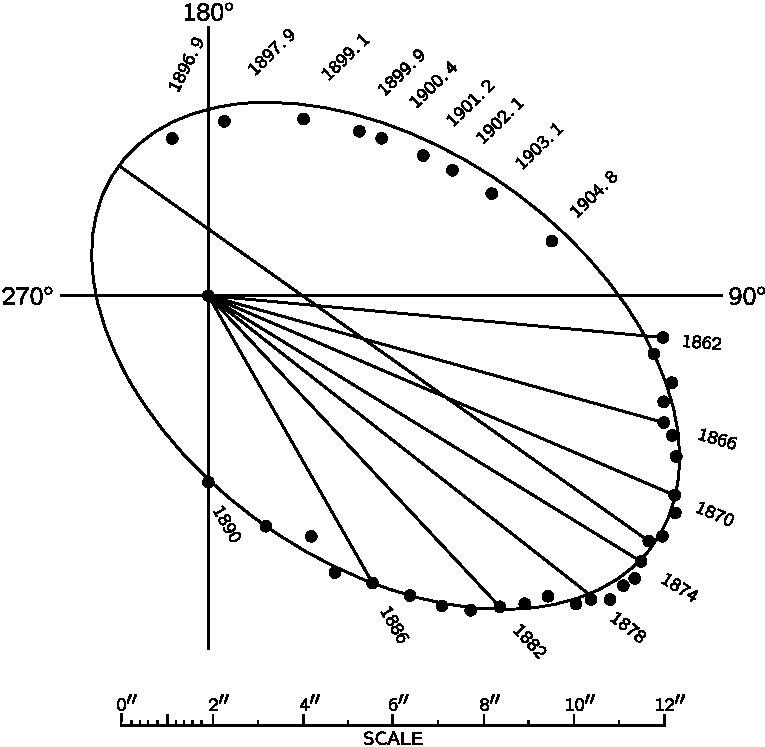
\includegraphics[width=0.8\linewidth]{fyz_fig0090.pdf}
      \caption{Dráha Síra B vzhledem k Síriu A (\cite[s.~99]{Feynman01})}
      \label{fyz:fig0090}
    \end{figure}

    Tento objev potvrzuje, že Newtonovy zákony jsou zcela správné v sluneční soustavě, ale zůstává 
    otázka, zda jsou správné i při větších vzdálenostech, než jsou relativně malé vzdáleností 
    nejbližších planet. Nejprve si můžeme položit otázku: Přitahují se hvězdy vzájemně také tak 
    jako planety? Přesvědčivý důkaz takové přitažlivostí máme v případě dvojhvězd Na obr. 
    \ref{fyz:fig0089} je vidět dvojhvězdu - dvě hvězdy, jež jsou velmi blízko u sebe (je tam i třetí 
    hvězda, a proto se můžeme přesvědčit, zda fotografie nebyla otočená). Obrázek nám ukazuje i 
    konfiguraci hvězd po několika letech. Je vidět, že vzhledem k \uv{pevné} hvězdě se osa páru 
    pootočila, tj. hvězdy obíhají jedna kolem druhé. Obíhají podle Newtonových zákonů? Pečlivá 
    měření relativních poloh jedné takové dvojhvězdy jsou zakreslena na obr. \ref{fyz:fig0090}. 
    Měření, která se uskutečnila mezi roky \num{1862} a \num{1904} (do dnešních dnů se musel 
    uskutečnit už i další oběh), dávají krásnou elipsu. Vše souhlasí s Newtonovými zákony, až na to 
    že hvězda Sírius A \emph{není v ohnisku}.  

    \begin{figure}[ht!]  %\ref{fyz:fig0092}
      \centering
      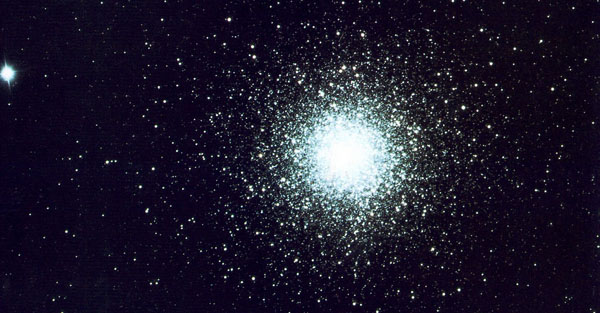
\includegraphics[width=\linewidth]{fyz_fig0092.jpg}
      \caption{Kulová hvězdokupa M 15 v souhvězdí Pegasa (\cite[s.~100]{Feynman01})}
      \label{fyz:fig0092}
    \end{figure}
    
    Proč dochází k něčemu takovému? Protože rovina elipsy není v \uv{rovině oblohy}. Na rovinu 
    dráhy se nedíváme pod pravým úhlem a když hledíme na nakloněnou elipsu, zůstane stále elipsou, 
    ale ohnisko nezůstane na původním místě. Tak můžeme relativní pohyb dvojhvězd analyzovat v 
    souladu s požadavky gravitačního zákona. 
    
    Pravdivost gravitačního zákona i na větších vzdálenostech potvrzuje obr. \ref{fyz:fig0092}. Jen 
    člověk bez představivosti na něm nevidí působení gravitace. Tento obrázek znázorňuje jednu z 
    nejkrásnějších věcí na obloze - kulovou hvězdokupu. Každá tečka je hvězda. Ačkoli hvězdy 
    vypadají, jako by byly pevně natlačeny k centru, jde pouze o nedokonalost našich přístrojů. Ve 
    skutečnosti jsou i vzdálenosti mezi středovými hvězdami velmi velké a jen velmi zřídka tu 
    dochází ke srážkám. Nejvíce hvězd je ve středu a se vzdalováním se od středu počet hvězd klesá. 
    Je zřejmé, že mezi těmito hvězdami existuje přitažlivost. 
    
    Je jasné, že na těchto ohromných vzdálenostech, \num{100000}-krát větších než je sluneční 
    soustava, existuje gravitační síla. Pojďme však dále a podívejme se na \emph{celou galaxii} 
    znázorněnou na obr. \ref{fyz:fig0093}. Tvar této galaxie svědčí o zjevné snaze její hmoty 
    aglomerovat. Samozřejmě nemůžeme dokázat, že tu jde přesně nepřímou úměrnost druhé mocnině 
    vzdálenosti, ale jen to, že i na těchto ohromných vzdálenostech je to přitažlivost, která drží 
    věci pohromadě. Je možné namítnout, že je to sice všechno pěkné, ale proč nemá galaxie kulový 
    tvar? Protože rotuje a má moment hybnosti, jehož se nemůže vzdát při smrštění; musí tedy být 
    smrštěna převážně v rovině. (Mimochodem, hledáme-li zajímavý problém, tak zatím nevíme, jak se 
    tvoří spirální ramena galaxie a co určuje tvar galaxií.) Je ale jasné, že tvar galaxie je určen 
    gravitací, i když složitost jeho struktury nám zatím brání úplně ho analyzovat. Rozměry galaxií 
    jsou asi od \num{50000} do \num{100000} světelných let. Jak velké jsou to vzdálenosti si 
    uvědomíme až tehdy, když uvážíme, že vzdálenost Země od Slunce je  \(8\tfrac{1}{3}\) světelných 
    minut. 
    
    \begin{figure}[ht!]  %\ref{fyz:fig0093}
      \centering
      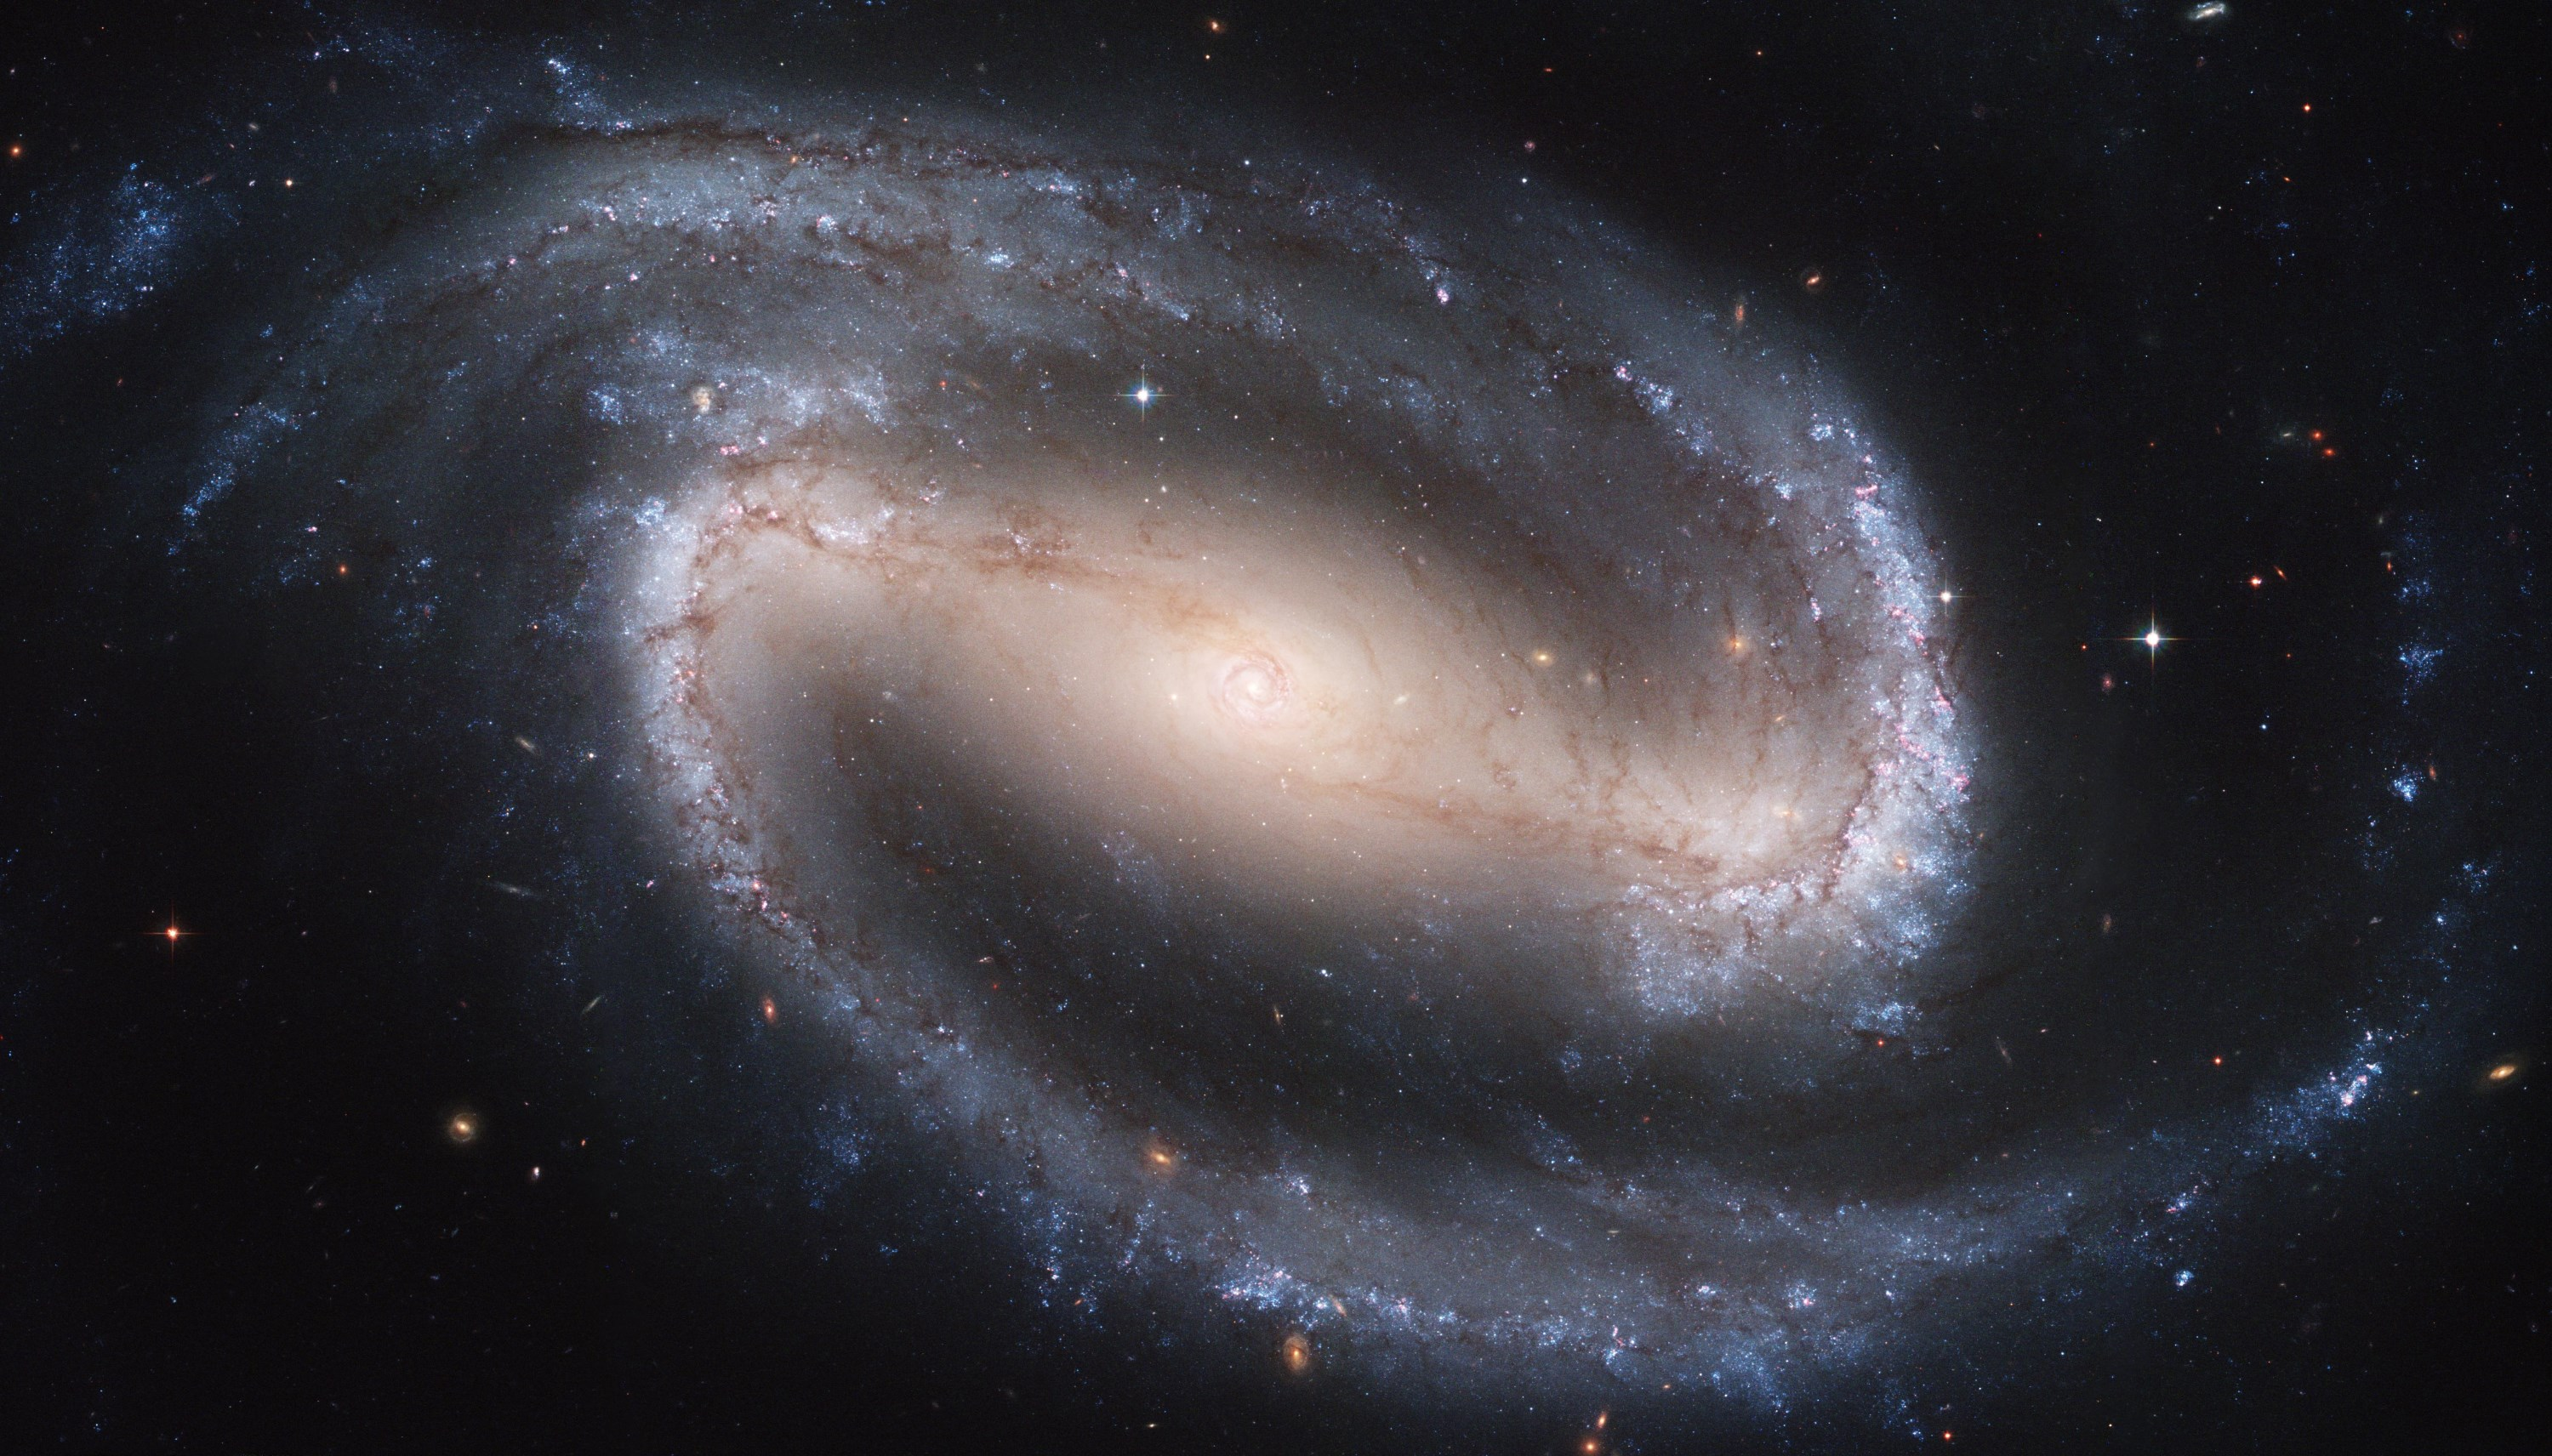
\includegraphics[width=\linewidth]{fyz_fig0093.jpg}
      \caption{Spirální galaxie s příčkou NGC 1300: Velká a krásná spirální galaxie s příčkou NGC
       1300 se nachází asi 70 miliónů světelných let daleko na březích řeky souhvězdí Eridanus.
       Kompozitní pohled z Hubblova kosmického dalekohledu na nádherný vesmírný ostrov je jedním z
       největších Hubblových snímků galaxie, který byl kdy pořízen. NGC 1300 měří přes 100 000
       světelných let a na Hubblovu snímku jsou vidět skvělé podrobnosti v dominantní centrální
       příčce i ve vznešených spirálních ramenech.  Podobně jako jiné spirální galaxie, včetně naší
       vlastní Mléčné dráhy, i u NGC 1300 se předpokládá, že má superhmotnou centrální černou díru.
       (\cite[s.~99]{Feynman01})}
      \label{fyz:fig0093}
    \end{figure}
    
    Zdá se, že přitažlivost existuje i ve větších vzdálenostech. Obr. \ref{fyz:fig0094} znázorňuje 
    shluk mnoha \uv{drobných} útvarů. Je to kupa \emph{galaxií}, podobná hvězdokupě. Galaxie se 
    tedy v takových vzdálenostech přitahují, a proto aglomerují do větších celků.

    \begin{figure}[ht!]  %\ref{fyz:fig0094}
      \centering
      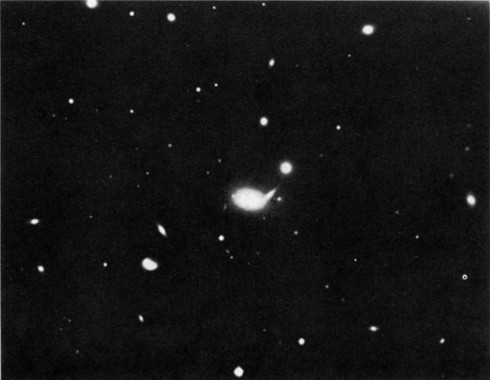
\includegraphics[width=0.8\linewidth]{fyz_fig0094.jpg}
      \caption{Kupa galaxií (\cite[s.~100]{Feynman01})}
      \label{fyz:fig0094}
    \end{figure}
    
    Gravitace snad existuje i ve vzdálenostech \emph{desítek miliónů} světelných let. Podle našich 
    dosavadních znalostí je gravitační síla všude nepřímo úměrná mocnině vzdálenosti. 

    \begin{figure}[ht!]  %\ref{fyz:fig0095}
      \centering
      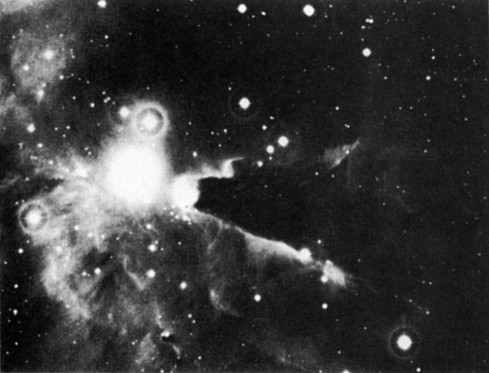
\includegraphics[width=0.8\linewidth]{fyz_fig0095.jpg}
      \caption{Mezihvězdný prachový oblak (\cite[s.~101]{Feynman01})}
      \label{fyz:fig0095}
    \end{figure}
    
    Gravitační zákon nám dovoluje pochopit nejen povahu mlhovin, ale poskytuje nám i určité 
    představy o původu hvězd. Máme-li velký oblak prachu a plynu podobný tomu, jenž je je znázorněn 
    na obr. \ref{fyz:fig0095}, vzájemná přitažlivost prachových částic může vyvolat jejich seskupení 
    do malých hrudek. Na obrázku slabě viditelné \uv{malé} černé skvrnky mohou být začátkem 
    akumulace prachu a plynů, které díky své přitažlivosti začínají tvořit hvězdy. Je diskutabilní, 
    zda jsme vůbec někdy viděli zrod hvězdy. Na obr. \ref{fyz:fig0096} je možná důkaz toho, že ano. 
    Na levé straně je obrázek oblasti plynu s několika hvězdami. Tento snímek pochází z roku 
    \num{1947}. Na pravé straně je obrázek o sem let mladší. Na něm jsou vidět dvě nové jasné 
    skvrny. Akumuloval se plyn a gravitace vyvolal jeho soustředění do dostatečně velké koule,takže 
    začala hvězdná jaderná reakce a přeměnila ho na hvězdu? Možná ano, možná ne. Je však 
    nepravděpodobné, že za pouhých sedm let bychom měli štěstí vidět přeměnu hvězdy do viditelné 
    podoby a ještě méně pravděpodobné je vidět takové přeměny hned dvě!

    \begin{figure}[ht!]  %\ref{fyz:fig0096}
      \centering
      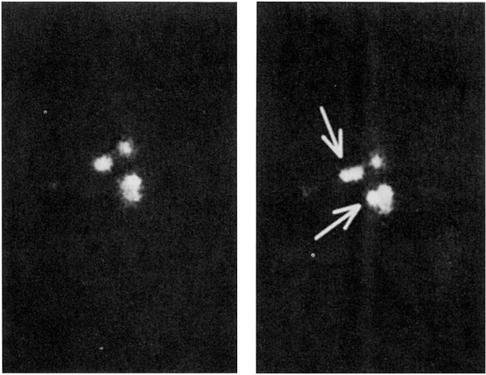
\includegraphics[width=0.8\linewidth]{fyz_fig0096.jpg}
      \caption{Vznik nových hvězd? (\cite[s.~101]{Feynman01})}
      \label{fyz:fig0096}
    \end{figure}
    
  \section{Cavendishův experiment}
    Gravitace tedy působí na obrovských vzdálenostech. Existuje-li však síla mezi 
    \emph{libovolnými} dvěma předměty, pak musí existovat možnost změřit tuto sílu působící mezi 
    předměty v našem okolí. Nemohli bychom namísto pozorování pohybu hvězd vzít olověnou a 
    mramorovou kuličku a pozorovat jak se bude pohybovat mramorová kulička k olověné? Obtížnost tak 
    jednoduchého experimentu spočívá v tom, že tato síla je sama velmi malá, jemná. Pokus je třeba 
    provádět s mimořádnou pečlivostí, což znamená vyčerpat vzduch z aparatury, vyloučit přítomnost 
    elektrických nábojů apod., a až potom je možné tu sílu měřit. Poprvé provedl takovéto měření 
    Cavendish na zařízení, které je schématicky znázorněno na obr. 7.13. Tímto pokusem se poprvé 
    dokazovala přímá síla mezi dvěma velkými pevnými olověnými koulemi a dvěma menšími olověnými 
    koulemi umístěnými na koncích vahadla upevněného na velmi jemném, tzv. torzním, vlákně. Měřením 
    zkroucení vlákna je možné měřit velikost síly a přesvědčit se, že je nepřímo úměrná druhé 
    mocnině vzdálenosti. Takto je možné přesně určit koeficient \(\kappa\) ve vztahu
    \begin{equation}\label{fyz:eq094}
      F = \kappa\frac{m_1m_2}{r^2}.
    \end{equation}
    
    \begin{figure}[ht!]  %\ref{fyz:fig0091}
      \centering
      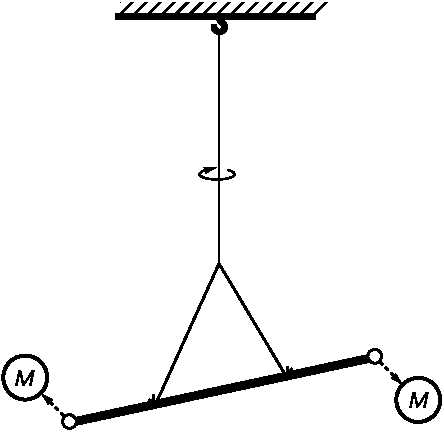
\includegraphics[width=0.5\linewidth]{fyz_fig0091.pdf}
      \caption{Zjednodušené schéma zařízení, pomocí něhož Cavendish ověřoval gravitační zákon v 
               případě malých objektů a měřil gravitační konstantu \(\kappa\)
               (\cite[s.~102]{Feynman01})}
      \label{fyz:fig0091}
    \end{figure}
    Všechny hmotnosti a vzdálenosti známe. Možná namítnete, že jsme je znali i v případě Země. Ano, 
    znali jsme vše, až na \emph{hmotnost Země}. Určením \(\kappa\) z tohoto experimentu a poznáním 
    zemské přitažlivosti můžeme nepřímo určit hmotnost Země! Tento experiment byl nazván „vážením 
    Země“. Cavendish tvrdil, že vážil Zemi, ale to, co skutečně měřil, byl koeficient \(\kappa\) 
    gravitačního zákona. To je jediný způsob jak je možné určit hmotnost Země.
    
    Koeficient \(\kappa\) je roven 
    \begin{equation}\label{fyz:eq095}
      \kappa = \qty{6.670e-11}{\N\square\meter\per\square\kg}.
    \end{equation}
    
    Je těžké přecenit důležitost vlivu velkého úspěchu gravitační teorie na historii vědy. Stačí 
    porovnat tehdejší zmatek, neúplné poznatky, nedůvěru, nekonečné debaty a paradoxy s jasností a 
    jednoduchostí tohoto zákona; s tím, že všechny měsíce, planety a hvězdy jsou \emph{ovládány tak 
    jednoduchým pravidlem}, kterému člověk \emph{rozumí} a umí z něho odvodit, jak se planety musí 
    pohybovat! V tom je třeba vidět příčinu úspěchu věd v následujících letech. Tento poznatek dal 
    lidem naději, že i jiné jevy mohou mít tak krásně jednoduché zákony.
    
  \section{Co je to gravitace?}
    Je to však skutečně tak jednoduchý zákon? Co je možné říci o jeho příčině? Dosud jsme jen 
    popisovali, \emph{jak} se Země pohybuje kolem Slunce, ale nehovořili jsme o tom, co 
    \emph{vyvolává tento pohyb}. Newton se vědomě nezabýval tímto problémem; nevymýšlel si 
    hypotézy. Uspokojil se s poznáním toho, co se odehrává, bez poznání mechanizmu. \emph{Dosud 
    však nikdo takový mechanizmus neobjevil}. Fyzikální zákony se vyznačují právě takovýmto 
    abstraktním charakterem. Zákon zachování energie je tvrzení týkající se veličin, jež je třeba 
    vypočítat a sčítat, a není v něm zmínky o mechanizmu. Podobně je to i s velkými zákony 
    mechaniky, které jsou kvantitativními matematickými zákony, jejichž vnitřní mechanizmus 
    neznáme. Proč k popisu přírody můžeme používat matematiku, aniž bychom věděli, jaký mechanizmus 
    se za tím skrývá? To neví nikdo. Musíme to dělat i nadále, neboť tak se můžeme více dozvědět.
    
    Bylo navrženo mnoho mechanizmů gravitace. Bude zajímavé si všimnout jednoho z nich, k němuž se 
    lidé čas od času vracejí. Zpočátku každý, kdo takovýto mechanizmus „objeví“, je vzrušený a 
    šťastný, ale brzy zjistí, že mechanizmus není správný. Poprvé byl objeven kolem roku 
    \num{1750}. Představte si, že v prostoru je velké množství částic, jež se pohybují velkou 
    rychlostí ve všech směrech a při průchodu hmotou jsou jen velmi málo absorbovány. Když jsou 
    absorbovány Zemí, ode vzdávají jí hybnost. Protože je těch, které letí jedním směrem, stejně 
    mnoho jako těch, které letí opačným směrem, hybnosti jsou vyvážené. Když se však přiblíží 
    Slunce, jsou částice přicházející na Zemi skrz Slunce částečně absorbovány a ve směru od Slunce 
    přichází méně částic než z opačné strany. Země proto získá hybnost směřující ke Slunci a nedá 
    mnoho práce zjistit, že síla bude nepřímo úměrná druhé mocnině vzdálenosti - tak se totiž se 
    vzdáleností mění prostorový úhel, pod nímž vidíme Slunce. Co je na tomto mechanizmu špatně? 
    Zahrnuje některé nové důsledky, které \emph{nejsou správné}. Taková myšlenka totiž vede k 
    následujícímu problému: Země by při svém pohybu kolem Slunce narážela na více částic zepředu 
    než zezadu. (Když běžíte v dešti, je déšť do tváře silnější než déšť do týla!). Země by proto 
    měla dostávat více hybnosti zepředu a měla by proto pociťovat \emph{odpor} a zpomalovat se. Je 
    možné spočítat, jaký čas by potřebovala Země k zastavení v důsledku takovéhoto odporu; ukazuje 
    se, že Země by se už měla pomalu zastavit, takže tento mechanizmus selhává. Zatím se nenašel 
    žádný mechanizmus, jenž by vysvětloval „gravitaci“ bez předpovězení jiných jevů, které však 
    \emph{neexistují}.
    
    Všimněme si ještě možného vztahu gravitace k jiným silám. Zatím neexistuje vysvětlení gravitace 
    pomocí jiných sil. Gravitace není projevem elektřiny nebo něčeho podobného, takže vysvětlení 
    nemáme. Gravitace je však jiným silám velmi podobná a je zajímavé blíže si všimnout této 
    podobnosti. Například elektrická síla mezi dvěma nabitými předměty připomíná gravitační zákon: 
    je rovna záporné konstantní veličině násobené součinem nábojů a mění se nepřímo úměrně s druhou 
    mocninou jejich vzdálenosti. Působí na opačnou stranu - způsobuje odpuzování. Není přece jen 
    velmi pozoruhodné, že tyto dva zákony obsahují stejnou funkci vzdálenosti? Možná, že mezi 
    gravitací a elektřinou je mnohem větší souvislost než si myslíme. Bylo uskutečněno mnoho pokusů 
    o sjednocení elektřiny a gravitace, takzvaná jednotná teorie pole je pouze velmi elegantním 
    pokusem zkombinovat elektřinu a gravitaci. Při porovnávání gravitace a elektřiny je 
    nejzajímavější \emph{relativní velikost} sil. Každá teorie, která je obsahuje obě dvě, musí 
    objasnit i velikost gravitace.
    
    Určíme-li v nějakých přirozených jednotkách odpuzování dvou elektronů (univerzální náboj 
    přírody) způsobené elektrickými silami a přitažlivost těchto elektronů způsobenou jejich 
    hmotnostmi, můžeme určit poměr elektrického odpuzování a gravitačního přitahování. Tento poměr 
    nezávisí na vzdálenosti a je základní konstantou přírody. Je znázorněn na obr. 
    \ref{fyz:fig0097}. Poměr gravitační přitažlivosti a elektrického odpuzování dvou elektronů je 
    1:\num{4.17e42}! Kde se vzalo tak velké číslo? Určitě není výsledkem náhody - vždyť nejde o 
    poměr velikosti Země a blechy. Uvažovali jsme dvě přirozené vlastnosti stejné věci - elektronu. 
    Toto fantastické číslo je přirozenou konstantou; skrývá v sobě jakési tajemství přírody. Jak se 
    mohlo tak ohromné číslo objevit? Jsou lidé, kteří tvrdí, že jednou objevíme „univerzální 
    rovnici“ a jedním z jejích kořenů bude právě toto číslo. Je však velmi těžké najít rovnici, 
    jejímž přirozeným kořenem by bylo tak fantastické číslo. Uvažovalo se i o jiných možnostech a 
    jedna z nich dává uvedené číslo do souvislosti s věkem vesmíru. Prostě musíme někde najít jiné 
    tak velké číslo. Ale máme na mysli věk vesmíru vyjádřený v rokách? Ne, protože roky nejsou 
    „přirozené“; ty vymyslel člověk. Jako příklad něčeho přirozeného uvažujme čas, za který světlo 
    projde protonem, tj. \qty{e-24}{\s}. Porovnáme-li tento čas s \textbf{věkem vesmíru}, který je 
    \num{2e10} let, dostaneme \num{e-42}. Protože má toto číslo přibližně stejný počet nul, byla 
    gravitační konstantě přisouzena souvislost s věkem vesmíru. Je-li to pravda, pak se gravitační 
    konstanta musí měnit s časem, neboť jak vesmír stárne, postupně roste poměr mezi jeho věkem a 
    časem, který potřebuje světlo k průchodu protonem. Je možné, že gravitační konstanta se 
    \emph{mění} s časem? Je jasné, že změny by byly tak malé, že přesvědčit se o nich by bylo velmi 
    obtížné.
    
    \begin{figure}[ht!]  %\ref{fyz:fig0097}
      \centering
      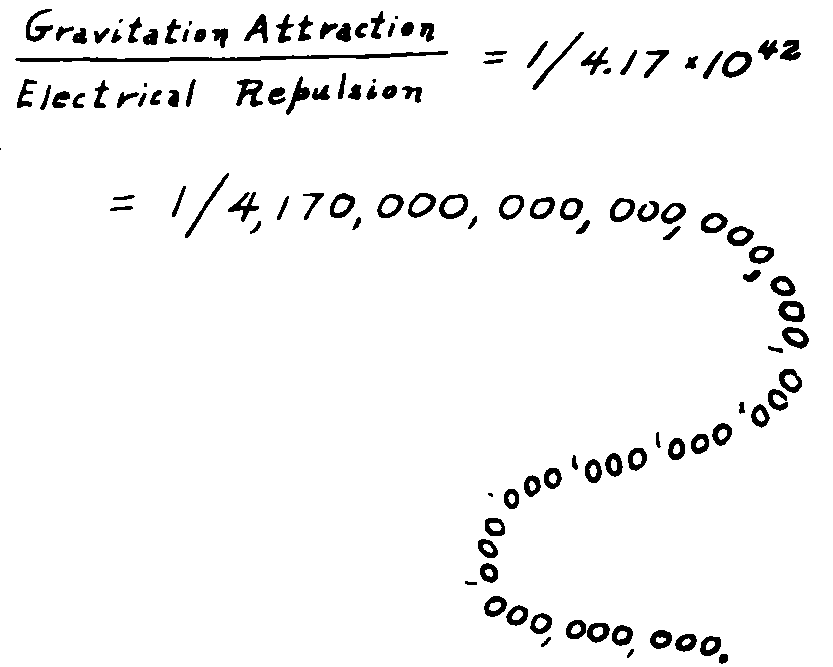
\includegraphics[width=0.7\linewidth]{fyz_fig0097.pdf}
      \caption{Relativní síla elektrické a gravitační interakce mezi dvěma elektrony
               (\cite[s.~104]{Feynman01})}
      \label{fyz:fig0097}
    \end{figure}
    Jedním ze způsobů ověření je zjistit, jaký vliv by měla změna gravitační konstanty v průběhu 
    posledních \num{e9} let, což představuje přibližně období od začátku života na Zemi až dodnes 
    nebo jednu desetinu stáří vesmíru. Za toto období by měla gravitační konstanta vzrůst asi o 
    10\%. Kdybychom uvažovali strukturu Slunce - rovnováhu mezi jeho hmotností a rychlostí, kterou 
    je v něm generována zářivá energie - dospěli bychom k závěru, že při gravitaci o 10\% větší by 
    mělo být Slunce mnohem více než o 10\% jasnější -jeho jas by měl růst se \emph{šestou mocninou} 
    gravitační konstanty! Kdybychom počítali, co se stane se zemskou orbitální dráhou při změně 
    gravitace, zjistili bychom, že Země by se k Slunci přiblížila. Výsledkem by byla teplota Země 
    asi o \qty{100} {\degreeCelsius} vyšší, takže voda by nebyla v mořích, ale ve formě vodních par 
    ve vzduchu, a v mořích by se nemohl vyvinout život. Proto dnes \emph{nevěříme}, že se 
    gravitační konstanta mění s věkem vesmíru. Ale naše argumentace není zcela přesvědčivá, a proto 
    není tento problém definitivně vyřešen.
    
    Skutečnost je taková, že síla gravitace je úměrná \emph{hmotnosti}, veličině, která je základní 
    mírou setrvačnosti - nebo mírou toho, jak těžké je udržet těleso pohybující se po kruhové 
    dráze. Proto dva předměty, jeden těžký a druhý lehký, obíhající kolem většího předmětu po 
    stejné kružnici stejnou rychlostí pod vlivem gravitace zůstanou stále spolu, protože pohyb po 
    kružnici si \emph{vyžaduje} pro větší hmotnost větší sílu. Jinak řečeno, gravitace je při větší 
    hmotnosti \emph{úměrněvě} větší, takže dva předměty se budou pohybovat spolu. Kdyby byl jeden 
    předmět uvnitř druhého, zůstal by tam; rovnováha je dokonalá. Proto Gagarin a Titov pozorovali 
    \uv{beztížnost} věcí uvnitř kosmické lodě; kdyby například vypustili kousek křídy, pohyboval by 
    se kolem Země stejným způsobem jako celá kosmická loď a jevil by se jim, jako kdyby visel před 
    nimi v prostoru. Je velmi zajímavé, že tato síla je	\emph{přesně} úměrná hmotnosti, protože v 
    opačném případě by musely existovat jevy, při nichž by se setrvačná a gravitační síla lišily. 
    Takový jev neexistuje, prověřil to s velkou přesností nejprve v roce \num{1909} E\"{o}tv\"{o}s 
    a později Dicke. Tyto pokusy vedly u všech použitých látek k úměrnosti hmotností a tíhy s 
    přesností 1:\num{1 000 000 000} nebo ještě lepší. Je to skutečně pozoruhodný experiment.
    
  \section{Gravitace a relativita}
    Další problém, který si zasluhuje pozornost, je Einsteinova modifikace Newtonova gravitačního 
    zákona. Navzdory nadšení, které Newtonův gravitační zákon vyvolal, není tento zákon správný! 
    Einstein ho pozměnil tak, aby vyhovoval požadavkům teorie relativity. Podle Newtona je 
    gravitační působení okamžité, tj. pohneme-li hmotností, měli bychom okamžitě pociťovat změnu 
    síly v důsledku změněné polohy této hmotnosti. Takovýmto způsobem by bylo možné posílat signály 
    nekonečnou rychlostí. Einstein předložil důvody, proč \emph{nemůžeme posílat signály větší 
    rychlostí než je rychlost světla}, takže gravitační zákon musí být chybný. Opravíme-li tento 
    zákon tak, že vezmeme v úvahu opožďování signálu, dostaneme nový zákon - nazývaný 
    \textbf{Einsteinův gravitační zákon}. Jedním snadno pochopitelným rysem tohoto nového zákona je 
    následující skutečnost. V Einsteinově teorii relativity vše co má \emph{energii}, má hmotnost - 
    hmotnost v tom smyslu, že je gravitačně přitahováno. Proto i světlo, které má energii, má 
    \uv{hmotnost}. Když světelný paprsek mající energii prochází kolem Slunce, působí na něho 
    přitažlivost Slunce. Světlo se proto nešíří přímo, ale ohýbá se. Například po dobu slunečních 
    zatmění se hvězdy, které jsou kolem Slunce, zdají posunuty z míst, kde by byly, kdyby Slunce 
    nebylo. To bylo skutečně pozorováno.

    \begin{figure}[ht!]  %\ref{fyz:fig0888}
      \centering
      \luafigure[1]{fyz_fig0888.jpg}
      \caption{ Jev gravitační čočky. Mezilehlý objekt (v tomto případě kupa galaxií) zdeformuje
                časoprostor natolik, že obraz vzdáleného objektu (v tomto případě galaxie) je
                zesílen a deformován. Kredit: CFHTLenS/NASA/ESA/Aldebaran.}
      \label{fyz:fig0888}
    \end{figure}
    
    Nakonec porovnejme gravitaci s jinými teoriemi. V posledních letech se zjistilo, že každá hmota 
    se skládá z nepatrných částic a že existují různé druhy interakcí, jako jaderné síly apod. 
    Žádná z těchto jaderných nebo elektrických sil však zatím nevysvětluje gravitaci.     
    Kvantově-mechanické aspekty přírody ještě nebyly rozšířeny na gravitaci. U velmi malých 
    rozměrů, kde dochází ke kvantovým jevům, je gravitační působení tak slabé, že zatím nevznikla 
    potřeba vytvořit kvantovou teorii gravitace. Kvůli důslednosti našich fyzikálních teorií by 
    však bylo důležité vědět, zda Newtonův zákon modifikovaný na Einsteinův zákon je možno dále 
    upravit tak, aby byl slučitelný s principem neurčitosti. Tato poslední úprava \emph{nebyla} 
    zatím dokončena.
  
  \section{Příklady a cvičení}

%} %tikzset
%---------------------------------------------------------------------------------------------------